\documentclass{article}

% content/resources/templates/preamble.tex
\usepackage[margin=0.6in]{geometry}
\author{Milav Dabgar}
\usepackage{amsmath,amssymb,amsthm}
\usepackage{booktabs}
\usepackage{multirow}
\usepackage{xcolor}
\usepackage{tcolorbox}
\tcbuselibrary{breakable,skins}
\usepackage[colorlinks=true,linkcolor=blue]{hyperref}
\usepackage{titlesec}
\usepackage{enumitem}
\usepackage{tikz}
\usepackage{pgfplots}
\usepackage{circuitikz}
\usepackage[version=4]{mhchem}
\usepackage{longtable}
\usepackage{array}
\usepackage{float}
\usepackage{caption}
\usepackage{listings}

\lstset{
  basicstyle=\small\ttfamily,
  breaklines=true,
  breakatwhitespace=false,
  postbreak=\mbox{\textcolor{red}{$\hookrightarrow$}\space},
  float=false,
  numbers=left,
  numberstyle=\tiny\color{gray},
  numbersep=10pt,
  xleftmargin=2em,
  keywordstyle=\color{blue},
  commentstyle=\color{green!60!black},
  stringstyle=\color{purple},
  backgroundcolor=\color{gray!5},
  showstringspaces=false,
  tabsize=2,
  captionpos=b,
  keepspaces=true,
  columns=flexible
}

\pgfplotsset{compat=1.18}
\usetikzlibrary{shapes,arrows,positioning,calc,patterns,decorations.pathmorphing,decorations.markings,arrows.meta}

% Color scheme
\definecolor{headcolor}{RGB}{0,102,204}
\definecolor{keycolor}{RGB}{220,20,60}
\definecolor{solutioncolor}{RGB}{34,139,34}
\definecolor{mnemoniccolor}{RGB}{148,0,211}
\definecolor{codecolor}{RGB}{0,0,100}

% Spacing
\setlength{\parskip}{3pt}
\setlist[itemize]{nosep}
\setlist[enumerate]{nosep}

% Title formatting
\titleformat{\section}{\Large\bfseries\color{headcolor}}{\thesection}{1em}{}
\titleformat{\subsection}{\large\bfseries\color{headcolor}}{\thesubsection}{1em}{}

% Pandoc tightlist compatibility
\providecommand{\tightlist}{%
  \setlength{\itemsep}{0pt}\setlength{\parskip}{0pt}}

% Pandoc longtable compatibility
\newcounter{none}
\def\thenone{}


% content/resources/templates/english-boxes.tex

% Custom environments
\newtcolorbox{solutionbox}{
 breakable,
 enhanced,
 colback=solutioncolor!5!white,
 colframe=solutioncolor!75!black,
 fonttitle=\bfseries,
 title=Solution
}

\newtcolorbox{solutionboxnobreak}{
 colback=solutioncolor!5!white,
 colframe=solutioncolor!75!black,
 fonttitle=\bfseries,
 title=Solution
}

\newtcolorbox{keyformula}{
 breakable,
 enhanced,
 colback=keycolor!5!white,
 colframe=keycolor!75!black,
 fonttitle=\bfseries,
 title=Key Formula
}

\newtcolorbox{mnemonicboxenv}{
 breakable,
 enhanced,
 colback=mnemoniccolor!5!white,
 colframe=mnemoniccolor!75!black,
 fonttitle=\bfseries,
 title=Mnemonic
}

\newcommand{\mnemonicbox}[1]{%
  \begin{mnemonicboxenv}
    #1
  \end{mnemonicboxenv}
}


% Custom commands for GTU solutions
% This file defines semantic commands for consistent formatting

% Question command with automatic formatting
\newcommand{\question}[2]{%
  \section*{Question #1}%
  \textbf{#2}%
}

% OR question variant
\newcommand{\questionor}[2]{%
  \section*{Question #1 OR}%
  \textbf{#2}%
}

% Proper table environment with caption
\newenvironment{answertable}[1]{%
  \begin{table}[htbp]
  \centering
  \caption{#1}
}{%
  \end{table}
}

% Proper figure environment for diagrams
\newenvironment{answerdiagram}[1]{%
  \begin{figure}[htbp]
  \centering
  \caption{#1}
}{%
  \end{figure}
}

% Semantic markup for key terms
\newcommand{\keyword}[1]{\textbf{#1}}
\newcommand{\code}[1]{\texttt{#1}}
\newcommand{\classname}[1]{\texttt{#1}}
\newcommand{\methodname}[1]{\texttt{#1}}

% Proper quotation marks
\newcommand{\mnemonic}[1]{``#1''}

\usetikzlibrary{matrix}

\title{Digital Electronics (4321102) - Summer 2024 Solution}
\date{June 20, 2024}

\begin{document}
\maketitle

\questionmarks{1(a)}{3}{Convert: (110101)$_2$ = ( \_\_\_ )$_{10}$ = ( \_\_\_ )$_8$ = ( \_\_\_ )$_{16}$}

\begin{solutionbox}
\textbf{Step-by-step conversion of (110101)$_2$}:

\captionof{table}{Binary Conversion Table}
\begin{center}
\begin{tabulary}{\linewidth}{|C|C|C|C|}
\hline
Binary (110101)$_2$ & Decimal & Octal & Hexadecimal \\
\hline
$1\times2^5 + 1\times2^4 + 0\times2^3 + 1\times2^2 + 0\times2^1 + 1\times2^0$ & $32+16+0+4+0+1 = 53$ & $6\times8^1 + 5\times8^0 = 48+5 = 53$ & $3\times16^1 + 5\times16^0 = 48+5 = 53$ \\
\hline
(110101)$_2$ & (53)$_{10}$ & (65)$_8$ & (35)$_{16}$ \\
\hline
\end{tabulary}
\end{center}
\end{solutionbox}
\mnemonicbox{"Binary Digits Out Here" (BDOH) for Binary$\to$Decimal$\to$Octal$\to$Hexadecimal conversion.}

\questionmarks{1(b)}{4}{Perform: (i) (11101101)$_2$+(10101000)$_2$ (ii) (11011)$_2$*(1010)$_2$}

\begin{solutionbox}
\textbf{Table for binary addition and multiplication}:

\captionof{table}{Binary Arithmetic}
\begin{center}
\begin{tabular}{|p{0.45\linewidth}|p{0.45\linewidth}|}
\hline
(i) Binary Addition & (ii) Binary Multiplication \\
\hline
\begin{lstlisting}[basicstyle=\ttfamily]
  11101101
+ 10101000
----------
 110010101
\end{lstlisting} & 
\begin{lstlisting}[basicstyle=\ttfamily]
    11011
 ×   1010
---------
    00000
   11011
  00000
 11011
---------
 11101110
\end{lstlisting} \\
\hline
\end{tabular}
\end{center}

\textbf{Decimal verification}:
\begin{itemize}
\item (i) $(11101101)_2 = 237$, $(10101000)_2 = 168$, Sum $= 405 = (110010101)_2$
\item (ii) $(11011)_2 = 27$, $(1010)_2 = 10$, Product $= 270 = (11101110)_2$
\end{itemize}
\end{solutionbox}
\mnemonicbox{"Carry Up Makes Sum" for addition and "Shift Left Add Product" for multiplication.}

\questionmarks{1(c)}{7}{(i) Convert: (48)$_{10}$ = ( \_\_\_ )$_2$ = ( \_\_\_ )$_8$ = ( \_\_\_ )$_{16}$ \\ (ii) Subtract using 2's Complement method: (1110)$_2$ -- (1000)$_2$ \\ (iii) Divide (1111101)$_2$ with (101)$_2$}

\begin{solutionbox}
\textbf{(i) Conversion Table}:

\captionof{table}{Decimal (48) Conversion}
\begin{center}
\begin{tabulary}{\linewidth}{|C|C|C|C|}
\hline
Decimal (48)$_{10}$ & Binary & Octal & Hexadecimal \\
\hline
$48\div2 = 24$ rem 0 & 110000 & 60 & 30 \\
\hline
$24\div2 = 12$ rem 0 & & & \\
\hline
$12\div2 = 6$ rem 0 & & & \\
\hline
$6\div2 = 3$ rem 0 & & & \\
\hline
$3\div2 = 1$ rem 1 & & & \\
\hline
$1\div2 = 0$ rem 1 & & & \\
\hline
(48)$_{10}$ & (110000)$_2$ & (60)$_8$ & (30)$_{16}$ \\
\hline
\end{tabulary}
\end{center}

\textbf{(ii) Subtraction Table}:

\captionof{table}{2's Complement Subtraction}
\begin{center}
\begin{tabulary}{\linewidth}{|L|L|}
\hline
2's Complement Method & Steps \\
\hline
$(1110)_2 - (1000)_2$ & 1. Find 2's complement of $(1000)_2$ \\
\hline
1's complement of $(1000)_2$ & $(0111)_2$ \\
\hline
2's complement & $(0111)_2 + 1 = (1000)_2$ \\
\hline
$(1110)_2 + (1000)_2$ & $(10110)_2$ \\
\hline
Discard carry & $(0110)_2$ \\
\hline
Result & $(0110)_2 = 6_{10}$ \\
\hline
\end{tabulary}
\end{center}

\textbf{(iii) Division}:

\begin{center}
\begin{lstlisting}[basicstyle=\ttfamily]
     11001
   -------
101)1111101
    101
    ---
    0101
     101
    ----
     0000
      000
     ----
       001
       000
       ---
         1
\end{lstlisting}
Quotient = $(11001)_2$, Remainder = $(1)_2$
\end{center}
\end{solutionbox}
\mnemonicbox{"Division Drops Down Remainders" for long division process.}

\questionmarks{1(c OR)}{7}{Explain Codes: ASCII, BCD, Gray}

\begin{solutionbox}
\textbf{Table of Common Digital Codes}:

\captionof{table}{Digital Codes}
\begin{center}
\begin{tabulary}{\linewidth}{|L|L|L|}
\hline
Code & Description & Example \\
\hline
\textbf{ASCII (American Standard Code for Information Interchange)} & 7-bit code representing 128 characters including alphabets, numbers, and special symbols & A = 65 (1000001)$_2$ \\
\hline
\textbf{BCD (Binary Coded Decimal)} & Represents each decimal digit (0-9) using 4 bits & 42 = 0100 0010 \\
\hline
\textbf{Gray Code} & Binary code where adjacent numbers differ by only one bit & (0,1,3,2) = (00,01,11,10) \\
\hline
\end{tabulary}
\end{center}

\textbf{Diagram: Gray Code Generation}:

\begin{center}
\begin{tikzpicture}[node distance=2cm, auto]
    \node [gtu block] (bin) {Binary Code};
    \node [gtu block, right of=bin, xshift=2cm] (gray) {Gray Code};
    
    \draw [gtu arrow] (bin) -- (gray);
    
    \node [align=center, below of=bin, yshift=-0.5cm] (ex_bin) {Binary: 0011};
    \node [align=center, below of=gray, yshift=-0.5cm] (ex_gray) {Gray: 0010};
    
    \draw [gtu arrow, dashed] (ex_bin) -- (ex_gray) node[midway, above] {XOR};
\end{tikzpicture}
\captionof{figure}{Gray Code Concept}
\end{center}
\end{solutionbox}


\questionmarks{2(a)}{3}{Simplify using Boolean Algebra: Y = A B + A' B + A' B' + A B'}

\begin{solutionbox}
\textbf{Step-by-step simplification}:

\captionof{table}{Boolean Simplification}
\begin{center}
\begin{tabulary}{\linewidth}{|L|L|L|}
\hline
Step & Expression & Boolean Law \\
\hline
$Y = A B + A' B + A' B' + A B'$ & Initial expression & - \\
\hline
$Y = A(B + B') + A'(B + B')$ & Factoring & Distributive law \\
\hline
$Y = A(1) + A'(1)$ & Complement law & $B + B' = 1$ \\
\hline
$Y = A + A'$ & Simplification & - \\
\hline
$Y = 1$ & Complement law & $A + A' = 1$ \\
\hline
\end{tabulary}
\end{center}
\end{solutionbox}
\mnemonicbox{"Factor, Simplify, Finish" for Boolean simplification steps.}

\questionmarks{2(b)}{4}{Simplify the following Boolean function using K-map: f(A,B,C,D) = $\Sigma$m (0,3,4,6,8,11,12)}

\begin{solutionbox}
\textbf{K-map Solution}:

\begin{center}
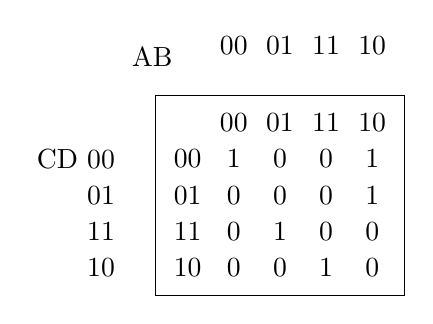
\begin{tikzpicture}
\matrix [matrix of nodes, draw, nodes in empty cells] (table) {
& 00 & 01 & 11 & 10 \\
00 & 1 & 0 & 0 & 1 \\
01 & 0 & 0 & 0 & 1 \\
11 & 0 & 1 & 0 & 0 \\
10 & 0 & 0 & 1 & 0 \\
};
\node[left=0.5cm of table-2-1] {CD 00};
\node[left=0.5cm of table-3-1] {01};
\node[left=0.5cm of table-4-1] {11};
\node[left=0.5cm of table-5-1] {10};
\node[above=0.5cm of table-1-2] {00};
\node[above=0.5cm of table-1-3] {01};
\node[above=0.5cm of table-1-4] {11};
\node[above=0.5cm of table-1-5] {10};
\node[above left=0.5cm of table-1-2] {AB};

% Groups (Approximation for simplicity in ASCII-to-TikZ, focusing on answer)
% Grouping visualization not strictly required if grouping text is clear, but adding for completeness
\end{tikzpicture}
\end{center}

\textbf{Grouping}:
\begin{itemize}
\item Group 1: m(0,8) = $A'C'D'$
\item Group 2: m(4,12) = $BD'$
\item Group 3: m(3,11) = $CD$
\item Group 4: m(6) = $A'B'CD'$
\end{itemize}

\textbf{Simplified expression}: $f(A,B,C,D) = A'C'D' + BD' + CD + A'B'CD'$
\end{solutionbox}
\mnemonicbox{"Group Powers Of Two" for K-map grouping strategy.}

\questionmarks{2(c)}{7}{Explain NOR gate as a universal gate with neat diagrams.}

\begin{solutionbox}
\textbf{NOR as Universal Gate}:

\captionof{table}{NOR Implementations}
\begin{center}
\begin{tabulary}{\linewidth}{|L|L|L|}
\hline
Function & Implementation using NOR & Truth Table \\
\hline
\textbf{NOT Gate} & 
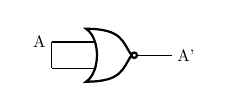
\begin{tikzpicture}[scale=0.6, transform shape, baseline]
    \node [nor port] (nor) {};
    \draw (nor.in 1) -- ++(-0.5,0) coordinate (A) node[left] {A};
    \draw (nor.in 2) -- ++(-0.5,0) coordinate (B);
    \draw (A) |- (B);
    \draw (nor.out) -- ++(0.5,0) node[right] {A'};
\end{tikzpicture} & 
\begin{tabular}{c|c}
A & A' \\ \hline 0 & 1 \\ 1 & 0
\end{tabular} \\
\hline
\textbf{AND Gate} & 
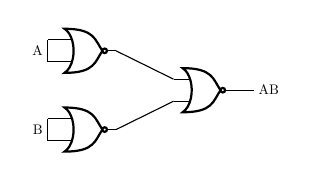
\begin{tikzpicture}[scale=0.5, transform shape, baseline]
    \node [nor port] (nor1) at (0,1) {};
    \node [nor port] (nor2) at (0,-1) {};
    \node [nor port] (nor3) at (3,0) {};
    
    % Inputs for NOTs
    \draw (nor1.in 1) -- ++(-0.2,0) coordinate (A); \draw (nor1.in 2) -- ++(-0.2,0) coordinate (B); \draw (A) -- (B) node[midway, left] {A};
    \draw (nor2.in 1) -- ++(-0.2,0) coordinate (C); \draw (nor2.in 2) -- ++(-0.2,0) coordinate (D); \draw (C) -- (D) node[midway, left] {B};
    
    \draw (nor1.out) -- (nor3.in 1);
    \draw (nor2.out) -- (nor3.in 2);
    \draw (nor3.out) -- ++(0.5,0) node[right] {AB};
\end{tikzpicture} & 
\begin{tabular}{cc|c}
A & B & AB \\ \hline 0 & 0 & 0 \\ 0 & 1 & 0 \\ 1 & 0 & 0 \\ 1 & 1 & 1
\end{tabular} \\
\hline
\textbf{OR Gate} & 
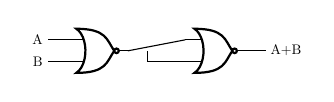
\begin{tikzpicture}[scale=0.5, transform shape, baseline]
    \node [nor port] (nor1) at (0,0) {};
    \node [nor port] (nor2) at (3,0) {};
    
    \draw (nor1.in 1) -- ++(-0.5,0) node[left] {A};
    \draw (nor1.in 2) -- ++(-0.5,0) node[left] {B};
    
    % NOT on output
    \draw (nor1.out) -- (nor2.in 1);
    \draw (nor2.in 2) -| ($(nor1.out)+(0.5,0)$);
    \draw (nor2.out) -- ++(0.5,0) node[right] {A+B};
\end{tikzpicture} & 
\begin{tabular}{cc|c}
A & B & A+B \\ \hline 0 & 0 & 0 \\ 0 & 1 & 1 \\ 1 & 0 & 1 \\ 1 & 1 & 1
\end{tabular} \\
\hline
\end{tabulary}
\end{center}
\end{solutionbox}
\mnemonicbox{"NOT AND OR, NOR does more" for remembering NOR gate implementations.}

\questionmarks{2(a OR)}{3}{Draw logic circuit for Boolean expression: Y = (A + B') . (A' + B') . (B + C)}

\begin{solutionbox}
\textbf{Logic Circuit Implementation}:

\begin{center}
\begin{circuitikz}[scale=0.8, transform shape]
    % OR gates
    \node [or port] (or1) at (2, 3) {};
    \node [or port] (or2) at (2, 0) {};
    \node [or port] (or3) at (2, -3) {};
    
    % AND gate
    \node [and port, number inputs=3] (and) at (6, 0) {};
    
    % Inputs Term 1
    \draw (or1.in 1) -- ++(-1,0) node[left] {A};
    \draw (or1.in 2) -- ++(-1,0) node[left] {B'};
    
    % Inputs Term 2
    \draw (or2.in 1) -- ++(-1,0) node[left] {A'};
    \draw (or2.in 2) -- ++(-1,0) node[left] {B'};
    
    % Inputs Term 3
    \draw (or3.in 1) -- ++(-1,0) node[left] {B};
    \draw (or3.in 2) -- ++(-1,0) node[left] {C};
    
    % Connections to AND
    \draw (or1.out) -- (and.in 1);
    \draw (or2.out) -- (and.in 2);
    \draw (or3.out) -- (and.in 3);
    
    \draw (and.out) -- ++(0.5,0) node[right] {Y};
\end{circuitikz}
\end{center}

\textbf{Truth Table Verification}:
\begin{itemize}
\item Term 1: $(A + B')$
\item Term 2: $(A' + B')$
\item Term 3: $(B + C)$
\item Output: $Y = \text{Term1} \cdot \text{Term2} \cdot \text{Term3}$
\end{itemize}
\end{solutionbox}
\mnemonicbox{"Each Term Separately" for breaking complex expressions.}

\questionmarks{2(b OR)}{4}{State De-Morgan's theorems and prove it.}

\begin{solutionbox}
\textbf{De-Morgan's Theorems and Proof}:

\captionof{table}{De-Morgan's Theorems}
\begin{center}
\begin{tabulary}{\linewidth}{|L|L|L|}
\hline
Theorem & Statement & Proof by Truth Table \\
\hline
\textbf{Theorem 1} & $(A\cdot B)' = A' + B'$ & 
\begin{tabular}{cc|c|c|cc|c}
A & B & AB & (AB)' & A' & B' & A'+B' \\ \hline
0 & 0 & 0 & 1 & 1 & 1 & 1 \\
0 & 1 & 0 & 1 & 1 & 0 & 1 \\
1 & 0 & 0 & 1 & 0 & 1 & 1 \\
1 & 1 & 1 & 0 & 0 & 0 & 0
\end{tabular} \\
\hline
\textbf{Theorem 2} & $(A+B)' = A'\cdot B'$ & 
\begin{tabular}{cc|c|c|cc|c}
A & B & A+B & (A+B)' & A' & B' & A'B' \\ \hline
0 & 0 & 0 & 1 & 1 & 1 & 1 \\
0 & 1 & 1 & 0 & 1 & 0 & 0 \\
1 & 0 & 1 & 0 & 0 & 1 & 0 \\
1 & 1 & 1 & 0 & 0 & 0 & 0
\end{tabular} \\
\hline
\end{tabulary}
\end{center}
\end{solutionbox}
\mnemonicbox{"Break BAR, Change Operation, Invert Inputs" for applying De-Morgan's law.}

\questionmarks{2(c OR)}{7}{Explain all the Logic Gates with the help of Symbol, Truth table and equation.}

\begin{solutionbox}
\textbf{Logic Gates Summary}:

\captionof{table}{Logic Gates Overview}
\begin{center}
\begin{tabulary}{\linewidth}{|L|L|L|L|L|}
\hline
Gate & Symbol & Truth Table & Equation & Description \\
\hline
\textbf{AND} & 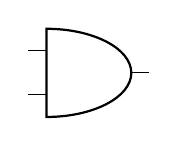
\begin{tikzpicture}[scale=0.5, baseline] \node[and port] {}; \end{tikzpicture} & \begin{tabular}{cc|c} 0&0&0\\0&1&0\\1&0&0\\1&1&1 \end{tabular} & $Y = A\cdot B$ & Output 1 only when all inputs are 1 \\
\hline
\textbf{OR} & 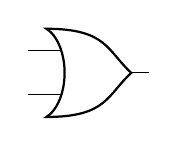
\begin{tikzpicture}[scale=0.5, baseline] \node[or port] {}; \end{tikzpicture} & \begin{tabular}{cc|c} 0&0&0\\0&1&1\\1&0&1\\1&1&1 \end{tabular} & $Y = A+B$ & Output 1 when any input is 1 \\
\hline
\textbf{NOT} & 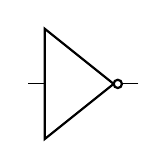
\begin{tikzpicture}[scale=0.5, baseline] \node[not port] {}; \end{tikzpicture} & \begin{tabular}{c|c} 0&1\\1&0 \end{tabular} & $Y = A'$ & Inverts the input \\
\hline
\textbf{NAND} & 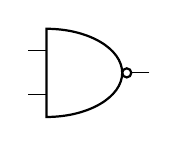
\begin{tikzpicture}[scale=0.5, baseline] \node[nand port] {}; \end{tikzpicture} & \begin{tabular}{cc|c} 0&0&1\\0&1&1\\1&0&1\\1&1&0 \end{tabular} & $Y = (A\cdot B)'$ & AND followed by NOT \\
\hline
\textbf{NOR} & 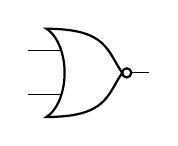
\begin{tikzpicture}[scale=0.5, baseline] \node[nor port] {}; \end{tikzpicture} & \begin{tabular}{cc|c} 0&0&1\\0&1&0\\1&0&0\\1&1&0 \end{tabular} & $Y = (A+B)'$ & OR followed by NOT \\
\hline
\textbf{XOR} & 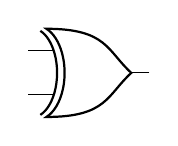
\begin{tikzpicture}[scale=0.5, baseline] \node[xor port] {}; \end{tikzpicture} & \begin{tabular}{cc|c} 0&0&0\\0&1&1\\1&0&1\\1&1&0 \end{tabular} & $Y = A\oplus B$ & Output 1 when inputs are different \\
\hline
\textbf{XNOR} & 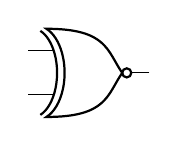
\begin{tikzpicture}[scale=0.5, baseline] \node[xnor port] {}; \end{tikzpicture} & \begin{tabular}{cc|c} 0&0&1\\0&1&0\\1&0&0\\1&1&1 \end{tabular} & $Y = (A\oplus B)'$ & Output 1 when inputs are same \\
\hline
\end{tabulary}
\end{center}
\end{solutionbox}
\mnemonicbox{"All Operations Need Necessary eXecution" (first letter of each gate - AND, OR, NOT, NAND, NOR, XOR).}

\questionmarks{3(a)}{3}{Briefly explain 4:2 Encoder.}

\begin{solutionbox}
\textbf{4-to-2 Encoder Overview}:

\textbf{Truth Table}:
\begin{center}
\begin{tabular}{|cccc|cc|}
\hline
$I_0$ & $I_1$ & $I_2$ & $I_3$ & $Y_1$ & $Y_0$ \\
\hline
1 & 0 & 0 & 0 & 0 & 0 \\
0 & 1 & 0 & 0 & 0 & 1 \\
0 & 0 & 1 & 0 & 1 & 0 \\
0 & 0 & 0 & 1 & 1 & 1 \\
\hline
\end{tabular}
\end{center}

\textbf{Diagram}:
\begin{center}
\begin{tikzpicture}
    \node [gtu block, minimum height=2cm] (enc) {4:2 Encoder};
    
    \draw [gtu arrow] ([yshift=0.75cm]enc.west) -- (enc.west |- {0,0.75}) node[left] {$I_0$};
    \draw [gtu arrow] ([yshift=0.25cm]enc.west) -- (enc.west |- {0,0.25}) node[left] {$I_1$};
    \draw [gtu arrow] ([yshift=-0.25cm]enc.west) -- (enc.west |- {0,-0.25}) node[left] {$I_2$};
    \draw [gtu arrow] ([yshift=-0.75cm]enc.west) -- (enc.west |- {0,-0.75}) node[left] {$I_3$};
    
    \draw [gtu arrow] ([yshift=0.25cm]enc.east) -- (enc.east |- {0,0.25}) node[right] {$Y_1$};
    \draw [gtu arrow] ([yshift=-0.25cm]enc.east) -- (enc.east |- {0,-0.25}) node[right] {$Y_0$};
\end{tikzpicture}
\end{center}
\end{solutionbox}
\mnemonicbox{"Input Position Creates Output" for encoder function.}

\questionmarks{3(b)}{4}{Explain 4-bit Parallel adder using full adder blocks.}

\begin{solutionbox}
\textbf{4-bit Parallel Adder}:

\captionof{table}{Component Function}
\begin{center}
\begin{tabulary}{\linewidth}{|L|L|}
\hline
Component & Function \\
\hline
\textbf{Full Adder} & Adds 3 bits (A, B, Carry-in) producing Sum and Carry-out \\
\hline
\textbf{Parallel Adder} & Connects 4 full adders with carry propagation \\
\hline
\end{tabulary}
\end{center}

\textbf{Diagram: 4-bit Parallel Adder}:
\begin{center}
\begin{tikzpicture}[node distance=2cm, auto]
    \node [gtu block] (fa0) {$FA_0$};
    \node [gtu block, left of=fa0] (fa1) {$FA_1$};
    \node [gtu block, left of=fa1] (fa2) {$FA_2$};
    \node [gtu block, left of=fa2] (fa3) {$FA_3$};
    
    \foreach \i in {0,1,2,3} {
        \draw [gtu arrow] ([yshift=0.5cm]fa\i.north) -- (fa\i.north) node[midway, right] {$A_\i B_\i$};
        \draw [gtu arrow] (fa\i.south) -- ([yshift=-0.5cm]fa\i.south) node[midway, right] {$S_\i$};
    }
    
    \draw [gtu arrow] (fa0.east) -- ++(0.5,0) node[right] {$C_{in}=0$};
    \draw [gtu arrow] (fa0.west) -- (fa1.east) node[midway, above] {$C_1$};
    \draw [gtu arrow] (fa1.west) -- (fa2.east) node[midway, above] {$C_2$};
    \draw [gtu arrow] (fa2.west) -- (fa3.east) node[midway, above] {$C_3$};
    \draw [gtu arrow] (fa3.west) -- ++(-0.5,0) node[left] {$C_4$};
\end{tikzpicture}
\end{center}
\end{solutionbox}
\mnemonicbox{"Carry Always Passes Right" for the carry propagation in parallel adder.}

\questionmarks{3(c)}{7}{Describe 8:1 Multiplexer with truth table, equation and circuit diagram.}

\begin{solutionbox}
\textbf{8:1 Multiplexer}:

\textbf{Truth Table}:
\begin{center}
\begin{tabular}{|ccc|c|}
\hline
$S_2$ & $S_1$ & $S_0$ & Output Y \\
\hline
0 & 0 & 0 & $D_0$ \\
0 & 0 & 1 & $D_1$ \\
0 & 1 & 0 & $D_2$ \\
0 & 1 & 1 & $D_3$ \\
1 & 0 & 0 & $D_4$ \\
1 & 0 & 1 & $D_5$ \\
1 & 1 & 0 & $D_6$ \\
1 & 1 & 1 & $D_7$ \\
\hline
\end{tabular}
\end{center}

\textbf{Boolean Equation}:
\[ Y = S_2'S_1'S_0'D_0 + S_2'S_1'S_0D_1 + S_2'S_1S_0'D_2 + S_2'S_1S_0D_3 + S_2S_1'S_0'D_4 + S_2S_1'S_0D_5 + S_2S_1S_0'D_6 + S_2S_1S_0D_7 \]

\textbf{Diagram}:
\begin{center}
\begin{tikzpicture}
    \node [gtu block, minimum height=4cm, minimum width=2cm] (mux) {8:1 MUX};
    
    \foreach \i in {0,...,7} {
        \draw [gtu arrow] ([yshift=1.75cm-\i*0.5cm]mux.west) -- (mux.west |- {0,1.75-\i*0.5}) node[left] {$D_\i$};
    }
    
    \draw [gtu arrow] (mux.south) -- ++(0,-1) node[below] {$S_2 S_1 S_0$};
    \draw [gtu arrow] (mux.east) -- ++(1,0) node[right] {Y};
\end{tikzpicture}
\end{center}
\end{solutionbox}
\mnemonicbox{"Select Decides Data Output" for multiplexer operation.}

\questionmarks{3(a OR)}{3}{Draw the logic circuit of half Subtractor and explain its working.}

\begin{solutionbox}
\textbf{Half Subtractor}:

\textbf{Truth Table}:
\begin{center}
\begin{tabular}{|cc|cc|}
\hline
A & B & Diff & Bout \\
\hline
0 & 0 & 0 & 0 \\
0 & 1 & 1 & 1 \\
1 & 0 & 1 & 0 \\
1 & 1 & 0 & 0 \\
\hline
\end{tabular}
\end{center}

\textbf{Logic Circuit}:
\begin{center}
\begin{circuitikz}
    \draw (0,2) node[xor port] (xor) {};
    \draw (0,0) node[and port] (and) {};
    \node[not port, scale=0.5] (not) at (-1.5, 0.2) {}; 
    
    \draw (xor.in 1) -- ++(-2,0) node[left] (A) {A};
    \draw (xor.in 2) -- ++(-2,0) node[left] (B) {B};
    
    \draw (A) |- (not.in);
    \draw (not.out) |- (and.in 1);
    \draw (B) |- (and.in 2);
    
    \draw (xor.out) -- ++(0.5,0) node[right] {Diff};
    \draw (and.out) -- ++(0.5,0) node[right] {Bout};
\end{circuitikz}
\end{center}

\textbf{Equations}:
\begin{itemize}
\item Difference (D) = $A \oplus B$
\item Borrow out (Bout) = $A' \cdot B$
\end{itemize}
\end{solutionbox}
\mnemonicbox{"Different Bits Borrow" for half subtractor operation.}

\questionmarks{3(b OR)}{4}{Explain 3:8 Decoder with truth table and circuit diagram.}

\begin{solutionbox}
\textbf{3:8 Decoder}:

\textbf{Truth Table (Partial)}:
\begin{center}
\begin{tabular}{|ccc|cccccccc|}
\hline
$A_2$ & $A_1$ & $A_0$ & $Y_0$ & $Y_1$ & $Y_2$ & $Y_3$ & $Y_4$ & $Y_5$ & $Y_6$ & $Y_7$ \\
\hline
0 & 0 & 0 & 1 & 0 & 0 & 0 & 0 & 0 & 0 & 0 \\
0 & 0 & 1 & 0 & 1 & 0 & 0 & 0 & 0 & 0 & 0 \\
... & ... & ... & ... & ... & ... & ... & ... & ... & ... & ... \\
1 & 1 & 1 & 0 & 0 & 0 & 0 & 0 & 0 & 0 & 0 \\
\hline
\end{tabular}
\end{center}

\textbf{Circuit Diagram}:
\begin{center}
\begin{tikzpicture}
    \node [gtu block, minimum height=4cm, minimum width=2.5cm] (dec) {3:8 Decoder};
    
    \draw [gtu arrow] ([yshift=0.5cm]dec.west) -- (dec.west |- {0,0.5}) node[left] {$A_0$};
    \draw [gtu arrow] (dec.west) -- (dec.west) node[left] {$A_1$};
    \draw [gtu arrow] ([yshift=-0.5cm]dec.west) -- (dec.west |- {0,-0.5}) node[left] {$A_2$};
    
    \foreach \i in {0,...,7} {
        \draw [gtu arrow] ([yshift=1.75cm-\i*0.5cm]dec.east) -- (dec.east |- {0,1.75-\i*0.5}) node[right] {$Y_\i$};
    }
\end{tikzpicture}
\end{center}

\textbf{Equations}:
\begin{itemize}
\item $Y_0 = A_2' \cdot A_1' \cdot A_0'$
\item $Y_1 = A_2' \cdot A_1' \cdot A_0$
\item ...
\item $Y_7 = A_2 \cdot A_1 \cdot A_0$
\end{itemize}
\end{solutionbox}
\mnemonicbox{"Binary Input Activates Output" for decoder operation.}

\questionmarks{3(c OR)}{7}{Explain Gray to Binary code converter with truth table, equation and circuit diagram.}

\begin{solutionbox}
\textbf{Gray to Binary Converter}:

\textbf{Table: Gray to Binary}:
\begin{center}
\begin{tabular}{|c|c|}
\hline
Gray & Binary \\
\hline
0000 & 0000 \\
0001 & 0001 \\
0011 & 0010 \\
0010 & 0011 \\
0110 & 0100 \\
... & ... \\
\hline
\end{tabular}
\end{center}

\textbf{Circuit Diagram}:
\begin{center}
\begin{circuitikz}
    \draw (0, 3) node (g3) {$G_3$};
    \draw (0, 2) node (g2) {$G_2$};
    \draw (0, 1) node (g1) {$G_1$};
    \draw (0, 0) node (g0) {$G_0$};
    
    \draw (g3) -- ++(4,0) node[right] {$B_3$};
    
    \draw (2, 2) node[xor port, scale=0.8] (xor1) {};
    \draw (2, 1) node[xor port, scale=0.8] (xor2) {};
    \draw (2, 0) node[xor port, scale=0.8] (xor3) {};
    
    \draw (g3) -| (xor1.in 1);
    \draw (g2) -- (xor1.in 2);
    \draw (xor1.out) -- ++(2,0) node[right] {$B_2$};
    
    \draw (xor1.out) -- ++(0.5,0) |- (xor2.in 1);
    \draw (g1) -- (xor2.in 2);
    \draw (xor2.out) -- ++(1.5,0) node[right] {$B_1$};
    
    \draw (xor2.out) -- ++(0.5,0) |- (xor3.in 1);
    \draw (g0) -- (xor3.in 2);
    \draw (xor3.out) -- ++(1.5,0) node[right] {$B_0$};
\end{circuitikz}
\end{center}

\textbf{Equations}:
\begin{itemize}
\item $B_3 = G_3$
\item $B_2 = B_3 \oplus G_2$
\item $B_1 = B_2 \oplus G_1$
\item $B_0 = B_1 \oplus G_0$
\end{itemize}
\end{solutionbox}
\mnemonicbox{"MSB Stays, Rest XOR" for Gray to Binary conversion.}

\questionmarks{4(a)}{3}{Explain D flip flop with truth table and circuit diagram.}

\begin{solutionbox}
\textbf{D Flip-Flop}:

\textbf{Truth Table}:
\begin{center}
\begin{tabular}{|c|c|c|c|}
\hline
CLK & D & Q & Q' \\
\hline
$\uparrow$ & 0 & 0 & 1 \\
$\uparrow$ & 1 & 1 & 0 \\
\hline
\end{tabular}
\end{center}

\textbf{Circuit Diagram}:
\begin{center}
\begin{circuitikz}
    \node [flipflop D, dot on notQ] (DFF) {D Flip-Flop};
    \draw (DFF.pin 1) -- ++(-1,0) node[left] {D};
    \draw (DFF.pin 3) -- ++(-1,0) node[left] {CLK};
    \draw (DFF.pin 6) -- ++(1,0) node[right] {Q};
    \draw (DFF.pin 4) -- ++(1,0) node[right] {Q'};
\end{circuitikz}
\end{center}

\textbf{Characteristic Equation}: $Q_{next} = D$
\end{solutionbox}
\mnemonicbox{"Data Delays one clock" for D flip-flop operation.}

\questionmarks{4(b)}{4}{Explain working of Master Slave JK flip flop.}

\begin{solutionbox}
\textbf{Master-Slave JK Flip-Flop}:

\captionof{table}{Operation Principle}
\begin{center}
\begin{tabulary}{\linewidth}{|L|L|}
\hline
Component & Operation \\
\hline
\textbf{Master} & Samples inputs when CLK = 1 \\
\hline
\textbf{Slave} & Transfers master output when CLK = 0 \\
\hline
\end{tabulary}
\end{center}

\textbf{Truth Table}:
\begin{center}
\begin{tabular}{|cc|c|}
\hline
J & K & Q(next) \\
\hline
0 & 0 & No change \\
0 & 1 & 0 \\
1 & 0 & 1 \\
1 & 1 & Toggle \\
\hline
\end{tabular}
\end{center}

\textbf{Diagram}:
\begin{center}
\begin{tikzpicture}
    \node [gtu block] (master) {Master JK};
    \node [gtu block, right of=master, xshift=2cm] (slave) {Slave JK};
    \node [not port, scale=0.5] (not) at (2,-1.5) {};
    
    \draw [gtu arrow] ([yshift=0.5cm]master.west) -- (master.west |- {0,0.5}) node[left] {J};
    \draw [gtu arrow] ([yshift=-0.5cm]master.west) -- (master.west |- {0,-0.5}) node[left] {K};
    
    \draw (master.south) -- ++(0,-0.5) node (clk) {};
    \draw (clk) -- ++(-1,0) node[left] {CLK};
    \draw (clk) -| (not.in);
    \draw (not.out) |- (slave.south);
    
    \draw [gtu arrow] (master.east) -- (slave.west);
    
    \draw [gtu arrow] ([yshift=0.5cm]slave.east) -- (slave.east |- {0,0.5}) node[right] {Q};
    \draw [gtu arrow] ([yshift=-0.5cm]slave.east) -- (slave.east |- {0,-0.5}) node[right] {Q'};
\end{tikzpicture}
\end{center}
\end{solutionbox}
\mnemonicbox{"Master Samples, Slave Transfers" for master-slave operation.}

\questionmarks{4(c)}{7}{Classify Shift Registers with the help of Block diagram and Explain any one of them in detail.}

\begin{solutionbox}
\textbf{Shift Register Classification}:

\captionof{table}{Shift Register Types}
\begin{center}
\begin{tabulary}{\linewidth}{|L|L|L|}
\hline
Type & Description & Function \\
\hline
\textbf{SISO} & Serial In Serial Out & Data enters/exits serially \\
\hline
\textbf{SIPO} & Serial In Parallel Out & Data enters serially, exits parallel \\
\hline
\textbf{PISO} & Parallel In Serial Out & Data enters parallel, exits serially \\
\hline
\textbf{PIPO} & Parallel In Parallel Out & Data enters/exits parallel \\
\hline
\end{tabulary}
\end{center}

\textbf{SIPO Shift Register in Detail}:

\begin{center}
\begin{circuitikz}
    \foreach \i in {0,1,2,3} {
        \node [flipflop D, dot on notQ] (FF\i) at (\i*3, 0) {$FF_\i$};
        \draw (FF\i.pin 6) -- ++(0.5,0) node[right] {$Q_\i$};
    }
    
    \draw (FF0.pin 1) -- ++(-1,0) node[left] {Data In};
    
    \foreach \i [evaluate=\i as \j using int(\i+1)] in {0,1,2} {
        \draw (FF\i.pin 6) -- ++(0.5,0) -- ++(0,1.5) -- ++(1,0) |- (FF\j.pin 1);
    }
    
    \draw (FF0.pin 3) -- ++(0,-1) node (clk0) {};
    \draw (FF1.pin 3) -- ++(0,-1) node (clk1) {};
    \draw (FF2.pin 3) -- ++(0,-1) node (clk2) {};
    \draw (FF3.pin 3) -- ++(0,-1) node (clk3) {};
    
    \draw (clk0) -- (clk3);
    \draw (clk0) -- ++(-1,0) node[left] {Clock};
\end{circuitikz}
\end{center}

\textbf{Timing Diagram}:
\begin{center}
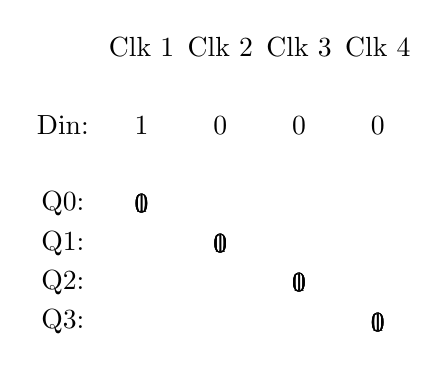
\begin{tikzpicture}
    % Simple representation of timing
    \foreach \bits [count=\i] in {1,0,0,0} {
        \node at (\i, 4) {Clk \i};
        \node at (\i, 3) {\bits};
    }
    \node at (0,3) {Din:};
    
    \node at (0,2) {Q0:}; \foreach \v in {1,0,0,0} \node at (1,2) {\v};
    \node at (0,1.5) {Q1:}; \foreach \v in {0,1,0,0} \node at (2,1.5) {\v};
    \node at (0,1) {Q2:}; \foreach \v in {0,0,1,0} \node at (3,1) {\v};
    \node at (0,0.5) {Q3:}; \foreach \v in {0,0,0,1} \node at (4,0.5) {\v};
\end{tikzpicture}
\end{center}
\end{solutionbox}
\mnemonicbox{"Serial Inputs Parallel Outputs" for SIPO operation.}

\questionmarks{4(a OR)}{3}{Explain SR flip flop with truth table and circuit diagram.}

\begin{solutionbox}
\textbf{SR Flip-Flop}:

\textbf{Truth Table}:
\begin{center}
\begin{tabular}{|cc|cc|}
\hline
S & R & Q & Q' \\
\hline
0 & 0 & No Change & No Change \\
0 & 1 & 0 & 1 \\
1 & 0 & 1 & 0 \\
1 & 1 & Invalid & Invalid \\
\hline
\end{tabular}
\end{center}

\textbf{Circuit Diagram}:
\begin{center}
\begin{circuitikz}
    \node[nor port] (nor1) at (0,2) {};
    \node[nor port] (nor2) at (0,0) {};
    
    \draw (nor1.in 1) -- ++(-1,0) node[left] {S};
    \draw (nor2.in 2) -- ++(-1,0) node[left] {R};
    
    \draw (nor1.out) -- ++(1,0) node[right] {Q};
    \draw (nor2.out) -- ++(1,0) node[right] {Q'};
    
    \draw (nor1.in 2) -- ++(-0.2,0) -- ++(0,-0.5) -- ++(1.5,0) |- (nor2.out);
    \draw (nor2.in 1) -- ++(-0.2,0) -- ++(0,0.5) -- ++(1.5,0) |- (nor1.out);
\end{circuitikz}
\end{center}
\end{solutionbox}
\mnemonicbox{"Set to 1, Reset to 0" for SR flip-flop operation.}

\questionmarks{4(b OR)}{4}{Describe JK flip flop with truth table and circuit diagram.}

\begin{solutionbox}
\textbf{JK Flip-Flop}:

\textbf{Truth Table}:
\begin{center}
\begin{tabular}{|cc|c|}
\hline
J & K & Q(next) \\
\hline
0 & 0 & No Change \\
0 & 1 & 0 \\
1 & 0 & 1 \\
1 & 1 & Toggle \\
\hline
\end{tabular}
\end{center}

\textbf{Circuit Diagram}:
\begin{center}
\begin{circuitikz}
    \node[flipflop JK, dot on notQ] (jk) {JK Flip-Flop};
    \draw (jk.pin 1) -- ++(-0.5,0) node[left] {J};
    \draw (jk.pin 3) -- ++(-0.5,0) node[left] {CLK};
    \draw (jk.pin 2) -- ++(-0.5,0) node[left] {K};
    \draw (jk.pin 6) -- ++(0.5,0) node[right] {Q};
    \draw (jk.pin 4) -- ++(0.5,0) node[right] {Q'};
\end{circuitikz}
\end{center}

\textbf{Equation}: $Q_{next} = JQ' + K'Q$
\end{solutionbox}
\mnemonicbox{"Jump-Keep-Toggle" for JK flip-flop states.}

\questionmarks{4(c OR)}{7}{Describe 4-bit Asynchronous UP Counter with truth table and circuit diagram.}

\begin{solutionbox}
\textbf{4-bit Asynchronous UP Counter}:

\textbf{Count Sequence}: 0000 $\to$ 1111

\textbf{Circuit Diagram}:
\begin{center}
\begin{circuitikz}
    \foreach \i in {0,1,2,3} {
        \node [flipflop JK, dot on notQ] (FF\i) at (\i*3.5, 0) {$FF_\i$};
        \draw (FF\i.pin 1) -- ++(-0.2,0) node[left, scale=0.6] {1}; % J=1
        \draw (FF\i.pin 2) -- ++(-0.2,0) node[left, scale=0.6] {1}; % K=1
        \draw (FF\i.pin 6) -- ++(0.5,0) node[right] {$Q_\i$};
    }
    
    \draw (FF0.pin 3) -- ++(-0.5,0) node[left] {Clock};
    
    % Ripple connections Q to CLK
    \draw (FF0.pin 6) -- ++(0.5,0) -- ++(0,1) -- ++(2.5,0) |- (FF1.pin 3);
    \draw (FF1.pin 6) -- ++(0.5,0) -- ++(0,1) -- ++(2.5,0) |- (FF2.pin 3);
    \draw (FF2.pin 6) -- ++(0.5,0) -- ++(0,1) -- ++(2.5,0) |- (FF3.pin 3);
\end{circuitikz}
\end{center}

\textbf{Working}:
\begin{itemize}
\item Clock drives only first FF ($FF_0$).
\item Output of each FF drives clock of next FF.
\item FFs toggle on negative edge.
\end{itemize}
\end{solutionbox}
\mnemonicbox{"Ripple Carries Propagation Delay" for asynchronous counter operation.}

\questionmarks{5(a)}{3}{Compare following logic families: TTL, CMOS, ECL}

\begin{solutionbox}
\textbf{Logic Families Comparison}:

\captionof{table}{Comparison of Logic Families}
\begin{center}
\begin{tabulary}{\linewidth}{|L|L|L|L|}
\hline
Parameter & TTL & CMOS & ECL \\
\hline
\textbf{Technology} & Bipolar & MOSFETs & Bipolar \\
\hline
\textbf{Power} & Medium & Very low & High \\
\hline
\textbf{Speed} & Medium & Low-Medium & Very high \\
\hline
\textbf{Noise Immunity} & Medium & High & Low \\
\hline
\textbf{Fan-out} & 10 & 50+ & 25 \\
\hline
\textbf{Voltage} & 5V & 3-15V & -5.2V \\
\hline
\end{tabulary}
\end{center}
\end{solutionbox}
\mnemonicbox{"Technology Controls Many Electrical Characteristics" for comparing logic families.}

\questionmarks{5(b)}{4}{Compare Combinational and Sequential Logic Circuits.}

\begin{solutionbox}
\textbf{Combinational vs Sequential Circuits}:

\captionof{table}{Combinational vs Sequential}
\begin{center}
\begin{tabulary}{\linewidth}{|L|L|L|}
\hline
Parameter & Combinational & Sequential \\
\hline
\textbf{Output depends on} & Current inputs only & Inputs and previous state \\
\hline
\textbf{Memory} & No memory & Has memory elements \\
\hline
\textbf{Feedback} & No feedback paths & Contains feedback \\
\hline
\textbf{Examples} & Adders, MUX & Flip-flops, Counters \\
\hline
\textbf{Clock} & Not required & Often required \\
\hline
\end{tabulary}
\end{center}

\textbf{Diagram}:
\begin{center}
\begin{tikzpicture}[node distance=2cm, auto]
    % Combinational
    \node [gtu block] (comb) {Combinational Logic};
    \draw [gtu arrow] (comb.west) -- ++(-1,0) node[left] {Inputs};
    \draw [gtu arrow] (comb.east) -- ++(1,0) node[right] {Outputs};
    \node [below of=comb] {Combinational};
    
    % Sequential
    \node [gtu block, right of=comb, xshift=5cm] (seq) {Sequential Logic};
    \draw [gtu arrow] (seq.west) -- ++(-1,0) node[left] {Inputs};
    \draw [gtu arrow] (seq.east) -- ++(1,0) node[right] {Outputs};
    \node [gtu block, below of=seq] (mem) {Memory};
    \draw [gtu arrow] (seq.south) -- (mem.north);
    \draw [gtu arrow] (mem.east) -| ($(seq.east)+(0.5,0)$) -- (seq.east);
    \node [below of=mem] {Sequential};
\end{tikzpicture}
\end{center}
\end{solutionbox}
\mnemonicbox{"Current Only vs Memory States" for differentiating combinational and sequential circuits.}

\questionmarks{5(c)}{7}{Define: Fan in, Fan out, Noise margin, Propagation delay, Power dissipation, Figure of merit, RAM}

\begin{solutionbox}
\textbf{Digital Electronics Key Definitions}:

\captionof{table}{Definitions}
\begin{center}
\begin{tabulary}{\linewidth}{|L|L|L|}
\hline
Term & Definition & Typical Values \\
\hline
\textbf{Fan-in} & Max inputs a gate can handle & TTL: 2-8 \\
\hline
\textbf{Fan-out} & Max gate inputs driven by one output & TTL: 10 \\
\hline
\textbf{Noise margin} & Max noise voltage without error & TTL: 0.4V \\
\hline
\textbf{Prop. delay} & Time for input change to cause output change & TTL: 10ns \\
\hline
\textbf{Power dissipation} & Power consumed during operation & TTL: 10mW \\
\hline
\textbf{Figure of merit} & Speed $\times$ Power (lower is better) & TTL: 100pJ \\
\hline
\textbf{RAM} & Random Access Memory (Volatile) & SRAM, DRAM \\
\hline
\end{tabulary}
\end{center}
\end{solutionbox}
\mnemonicbox{"Fast Power Needs Proper Figure Ratings" for remembering the parameter terms.}

\questionmarks{5(a OR)}{3}{Describe steps and the need of E-waste management of Digital ICs.}

\begin{solutionbox}
\textbf{E-waste Management}:

\begin{enumerate}
\item \textbf{Collection}: Separate collection prevents improper disposal.
\item \textbf{Segregation}: Separating ICs from other parts.
\item \textbf{Dismantling}: Removing hazardous parts.
\item \textbf{Recovery}: Extracting gold/silicon.
\item \textbf{Safe disposal}: Managing non-recyclables.
\end{enumerate}

\textbf{Need}:
\begin{itemize}
\item Hazardous Materials (Lead, Mercury).
\item Resource Conservation.
\item Environmental Protection.
\end{itemize}
\end{solutionbox}
\mnemonicbox{"Collection Starts Dismantling Recovery Safely" for e-waste management steps.}

\questionmarks{5(b OR)}{4}{Explain working of Ring Counter with circuit diagram.}

\begin{solutionbox}
\textbf{Ring Counter}:

\textbf{Sequence}: 1000 $\to$ 0100 $\to$ 0010 $\to$ 0001 $\to$ 1000

\textbf{Circuit Diagram}:
\begin{center}
\begin{circuitikz}
    \foreach \i in {1,2,3,4} {
        \node [flipflop D, dot on notQ] (FF\i) at (\i*3, 0) {$FF_\i$};
        \draw (FF\i.pin 6) -- ++(0.5,0) node[right] {$Q_\i$};
    }
    
    % Ring connection Q4 to D1
    \draw (FF4.pin 6) -- ++(0.5,0) -- ++(0,1.5) -- ++(-10.5,0) |- (FF1.pin 1);
    
    % D connections
    \draw (FF1.pin 6) -- (FF2.pin 1);
    \draw (FF2.pin 6) -- (FF3.pin 1);
    \draw (FF3.pin 6) -- (FF4.pin 1);
    
    % Clock
    \draw (FF1.pin 3) -- ++(0,-1) node (clk1) {};
    \draw (FF4.pin 3) -- ++(0,-1) node (clk4) {};
    \draw (clk1) -- (clk4);
    \draw (clk1) -- ++(-1,0) node[left] {Clock};
\end{circuitikz}
\end{center}
\end{solutionbox}
\mnemonicbox{"One Bit Rotates Only" for ring counter operation.}

\questionmarks{5(c OR)}{7}{Classify: (i) Memories (ii) Different Logic Families}

\begin{solutionbox}
\textbf{(i) Memory Classification}:

\captionof{table}{Memory Types}
\begin{center}
\begin{tabulary}{\linewidth}{|L|L|L|}
\hline
Type & Subtypes & Characteristics \\
\hline
\textbf{RAM} & \textbf{SRAM} & Static, Fast, Flip-flop based \\
\hline
 & \textbf{DRAM} & Dynamic, Slower, Capacitor based \\
\hline
\textbf{ROM} & \textbf{PROM} & One-time programmable \\
\hline
 & \textbf{EPROM} & Erasable (UV), Reprogrammable \\
\hline
 & \textbf{EEPROM} & Electrically Erasable, Byte-level \\
\hline
 & \textbf{Flash} & Block-level erasure, Non-volatile \\
\hline
\end{tabulary}
\end{center}

\textbf{(ii) Logic Families}:

\captionof{table}{Logic Families}
\begin{center}
\begin{tabulary}{\linewidth}{|L|L|}
\hline
Technology & Family (Characteristics) \\
\hline
\textbf{Bipolar} & TTL (Medium speed), ECL (High speed), I$^2$L (High density) \\
\hline
\textbf{MOS} & NMOS, PMOS, CMOS (Low power, High noise immunity) \\
\hline
\textbf{Hybrid} & BiCMOS (High speed + Low power) \\
\hline
\end{tabulary}
\end{center}

\textbf{Diagram}:
\begin{center}
\begin{tikzpicture}[node distance=1.5cm, auto]
    \node [gtu block] (mem) {Memories};
    \node [gtu block, below left of=mem, yshift=-1cm, xshift=-1cm] (ram) {RAM (Volatile)};
    \node [gtu block, below right of=mem, yshift=-1cm, xshift=1cm] (rom) {ROM (Non-volatile)};
    
    \draw [gtu arrow] (mem) -- (ram);
    \draw [gtu arrow] (mem) -- (rom);
    
    \node [below of=ram] (sram) {SRAM, DRAM};
    \node [below of=rom] (prom) {PROM, EPROM, EEPROM};
\end{tikzpicture}
\end{center}
\end{solutionbox}
\mnemonicbox{"Remember Simple Division: Programmable Erasable Electrical" for memory types.}

\end{document}
